\documentclass[journal,12pt,twocolumn]{IEEEtran}
%
\usepackage{setspace}
\usepackage{gensymb}
\usepackage{xcolor}
\usepackage{caption}
%\usepackage{subcaption}
%\doublespacing
\singlespacing

%\usepackage{graphicx}
%\usepackage{amssymb}
%\usepackage{relsize}
\usepackage[cmex10]{amsmath}
\usepackage{mathtools}
%\usepackage{amsthm}
%\interdisplaylinepenalty=2500
%\savesymbol{iint}
%\usepackage{txfonts}
%\restoresymbol{TXF}{iint}
%\usepackage{wasysym}
\usepackage{hyperref}
\usepackage{amsthm}
\usepackage{mathrsfs}
\usepackage{txfonts}
\usepackage{stfloats}
\usepackage{cite}
\usepackage{cases}
\usepackage{subfig}
%\usepackage{xtab}
\usepackage{longtable}
\usepackage{multirow}
%\usepackage{algorithm}
%\usepackage{algpseudocode}
%\usepackage{enumerate}
\usepackage{enumitem}
\usepackage{mathtools}
%\usepackage{iithtlc}
%\usepackage[framemethod=tikz]{mdframed}
\usepackage{listings}


%\usepackage{stmaryrd}


%\usepackage{wasysym}
%\newcounter{MYtempeqncnt}
\DeclareMathOperator*{\Res}{Res}
%\renewcommand{\baselinestretch}{2}
\renewcommand\thesection{\arabic{section}}
\renewcommand\thesubsection{\thesection.\arabic{subsection}}
\renewcommand\thesubsubsection{\thesubsection.\arabic{subsubsection}}

\renewcommand\thesectiondis{\arabic{section}}
\renewcommand\thesubsectiondis{\thesectiondis.\arabic{subsection}}
\renewcommand\thesubsubsectiondis{\thesubsectiondis.\arabic{subsubsection}}

%\renewcommand{\labelenumi}{\textbf{\theenumi}}
%\renewcommand{\theenumi}{P.\arabic{enumi}}

% correct bad hyphenation here
\hyphenation{op-tical net-works semi-conduc-tor}

\lstset{
language=Python,
frame=single, 
breaklines=true,
columns=fullflexible
}



\begin{document}
%

\theoremstyle{definition}
\newtheorem{theorem}{Theorem}[section]
\newtheorem{problem}{Problem}
\newtheorem{proposition}{Proposition}[section]
\newtheorem{lemma}{Lemma}[section]
\newtheorem{corollary}[theorem]{Corollary}
\newtheorem{example}{Example}[section]
\newtheorem{definition}{Definition}[section]
%\newtheorem{algorithm}{Algorithm}[section]
%\newtheorem{cor}{Corollary}
\newcommand{\BEQA}{\begin{eqnarray}}
\newcommand{\EEQA}{\end{eqnarray}}
\newcommand{\define}{\stackrel{\triangle}{=}}
\newcommand{\myvec}[1]{\ensuremath{\begin{pmatrix}#1\end{pmatrix}}}
\bibliographystyle{IEEEtran}
%\bibliographystyle{ieeetr}
\let\vec\mathbf
\providecommand{\nCr}[2]{\,^{#1}C_{#2}} % nCr
\providecommand{\nPr}[2]{\,^{#1}P_{#2}} % nPr
\providecommand{\mbf}{\mathbf}
\providecommand{\pr}[1]{\ensuremath{\Pr\left(#1\right)}}
\providecommand{\qfunc}[1]{\ensuremath{Q\left(#1\right)}}
\providecommand{\sbrak}[1]{\ensuremath{{}\left[#1\right]}}
\providecommand{\lsbrak}[1]{\ensuremath{{}\left[#1\right.}}
\providecommand{\rsbrak}[1]{\ensuremath{{}\left.#1\right]}}
\providecommand{\brak}[1]{\ensuremath{\left(#1\right)}}
\providecommand{\lbrak}[1]{\ensuremath{\left(#1\right.}}
\providecommand{\rbrak}[1]{\ensuremath{\left.#1\right)}}
\providecommand{\cbrak}[1]{\ensuremath{\left\{#1\right\}}}
\providecommand{\lcbrak}[1]{\ensuremath{\left\{#1\right.}}
\providecommand{\rcbrak}[1]{\ensuremath{\left.#1\right\}}}
\theoremstyle{remark}
\newtheorem{rem}{Remark}
\newcommand{\sgn}{\mathop{\mathrm{sgn}}}
\providecommand{\abs}[1]{\left\vert#1\right\vert}
\providecommand{\res}[1]{\Res\displaylimits_{#1}} 
\providecommand{\norm}[1]{\lVert#1\rVert}
\providecommand{\mtx}[1]{\mathbf{#1}}
\providecommand{\mean}[1]{E\left[ #1 \right]}
\providecommand{\fourier}{\overset{\mathcal{F}}{ \rightleftharpoons}}
\providecommand{\ztrans}{\overset{\mathcal{Z}}{ \rightleftharpoons}}

%\providecommand{\hilbert}{\overset{\mathcal{H}}{ \rightleftharpoons}}
\providecommand{\system}{\overset{\mathcal{H}}{ \longleftrightarrow}}
	%\newcommand{\solution}[2]{\textbf{Solution:}{#1}}
\newcommand{\solution}{\noindent \textbf{Solution: }}
\providecommand{\dec}[2]{\ensuremath{\overset{#1}{\underset{#2}{\gtrless}}}}
\numberwithin{equation}{section}
%\numberwithin{equation}{subsection}
%\numberwithin{problem}{subsection}
%\numberwithin{definition}{subsection}
\makeatletter
\@addtoreset{figure}{problem}
\makeatother

\let\StandardTheFigure\thefigure
%\renewcommand{\thefigure}{\theproblem.\arabic{figure}}
\renewcommand{\thefigure}{\theproblem}


%\numberwithin{figure}{subsection}

\def\putbox#1#2#3{\makebox[0in][l]{\makebox[#1][l]{}\raisebox{\baselineskip}[0in][0in]{\raisebox{#2}[0in][0in]{#3}}}}
     \def\rightbox#1{\makebox[0in][r]{#1}}
     \def\centbox#1{\makebox[0in]{#1}}
     \def\topbox#1{\raisebox{-\baselineskip}[0in][0in]{#1}}
     \def\midbox#1{\raisebox{-0.5\baselineskip}[0in][0in]{#1}}

\vspace{3cm}

\title{ 
%\logo{
Digital Signal Processing
%}
%	\logo{Octave for Math Computing }
}
%\title{
%	\logo{Matrix Analysis through Octave}{\begin{center}\includegraphics[scale=.24]{tlc}\end{center}}{}{HAMDSP}
%}


% paper title
% can use linebreaks \\ within to get better formatting as desired
%\title{Matrix Analysis through Octave}
%
%
% author names and IEEE memberships
% note positions of commas and nonbreaking spaces ( ~ ) LaTeX will not break
% a structure at a ~ so this keeps an author's name from being broken across
% two lines.
% use \thanks{} to gain access to the first footnote area
% a separate \thanks must be used for each paragraph as LaTeX2e's \thanks
% was not built to handle multiple paragraphs
%

\author{I Sai Pradeep% <-this % stops a space
%\thanks{J. Doe and J. Doe are with Anonymous University.}% <-this % stops a space
%\thanks{Manuscript received April 19, 2005; revised January 11, 2007.}}
}
% note the % following the last \IEEEmembership and also \thanks - 
% these prevent an unwanted space from occurring between the last author name
% and the end of the author line. i.e., if you had this:
% 
% \author{....lastname \thanks{...} \thanks{...} }
%                     ^------------^------------^----Do not want these spaces!
%
% a space would be appended to the last name and could cause every name on that
% line to be shifted left slightly. This is one of those "LaTeX things". For
% instance, "\textbf{A} \textbf{B}" will typeset as "A B" not "AB". To get
% "AB" then you have to do: "\textbf{A}\textbf{B}"
% \thanks is no different in this regard, so shield the last } of each \thanks
% that ends a line with a % and do not let a space in before the next \thanks.
% Spaces after \IEEEmembership other than the last one are OK (and needed) as
% you are supposed to have spaces between the names. For what it is worth,
% this is a minor point as most people would not even notice if the said evil
% space somehow managed to creep in.



% The paper headers
%\markboth{Journal of \LaTeX\ Class Files,~Vol.~6, No.~1, January~2007}%
%{Shell \MakeLowercase{\textit{et al.}}: Bare Demo of IEEEtran.cls for Journals}
% The only time the second header will appear is for the odd numbered pages
% after the title page when using the twoside option.
% 
% *** Note that you probably will NOT want to include the author's ***
% *** name in the headers of peer review papers.                   ***
% You can use \ifCLASSOPTIONpeerreview for conditional compilation here if
% you desire.




% If you want to put a publisher's ID mark on the page you can do it like
% this:
%\IEEEpubid{0000--0000/00\$00.00~\copyright~2007 IEEE}
% Remember, if you use this you must call \IEEEpubidadjcol in the second
% column for its text to clear the IEEEpubid mark.



% make the title area
\maketitle

%\newpage

\tableofcontents

%\renewcommand{\thefigure}{\thesection.\theenumi}
%\renewcommand{\thetable}{\thesection.\theenumi}

\renewcommand{\thefigure}{\theenumi}
\renewcommand{\thetable}{\theenumi}

%\renewcommand{\theequation}{\thesection}


\bigskip

\begin{abstract}
This manual provides a simple introduction to digital signal processing.
\end{abstract}
\section{Software Installation}
Run the following commands
\begin{lstlisting}
sudo apt-get update
sudo apt-get install libffi-dev libsndfile1 python3-scipy  python3-numpy python3-matplotlib 
sudo pip install cffi pysoundfile 
\end{lstlisting}
\section{Digital Filter}
\begin{enumerate}[label=\thesection.\arabic*
,ref=\thesection.\theenumi]
\item
\label{prob:input}
Download the sound file from  
\begin{lstlisting}
wget https://github.com/Pradeep8802/EE3900-Digital-Signal-Processing/blob/main/Assignment1/codes/Sound_Noise.wav
\end{lstlisting}
%\href{http://tlc.iith.ac.in/img/sound/Sound_Noise.wav}{\url{http://tlc.iith.ac.in/img/sound/Sound_Noise.wav}}  
%in the link given below.
%\linebreak
\item
\label{prob:spectrogram}
You will find a spectrogram at \href{https://academo.org/demos/spectrum-analyzer}{\url{https://academo.org/demos/spectrum-analyzer}}. 
%\end{problem}
%%
%
%%\onecolumn
%%\input{./figs/fir}
%\begin{problem}
Upload the sound file that you downloaded in Problem \ref{prob:input} in the spectrogram  and play.  Observe the spectrogram. What do you find?
\\
%
\solution There are a lot of yellow lines between 440 Hz to 5.1 KHz.  These represent the synthesizer key tones. Also, the key strokes
are audible along with background noise.
% By observing spectrogram, it clearly shows that tonal frequency is under 4kHz. And above 4kHz only noise is present.
\item
\label{prob:output}
Write the python code for removal of out of band noise and execute the code.
\\
\solution
\lstinputlisting{./codes/Cancel_noise.py}
%\begin{figure}[h]
%\centering
%\includegraphics[width=\columnwidth]{enc_block_diag.png}
%\caption{}
%\label{fig:convolution encoder}
%\end{figure}
%\input{block_enc}
\item
The output of the python script in Problem \ref{prob:output} is the audio file Sound\_With\_ReducedNoise.wav. Play the file in the spectrogram in Problem \ref{prob:spectrogram}. What do you observe?
\\
\solution The key strokes as well as background noise is subdued in the audio.  Also,  the signal is blank for frequencies above 5.1 kHz.

\end{enumerate}
\section{Difference Equation}
\begin{enumerate}[label=\thesection.\arabic*,ref=\thesection.\theenumi]
\item Let
\label{def:xn}
\begin{equation}
x(n) = \cbrak{\underset{\uparrow}{1},2,3,4,2,1}
\end{equation}
Sketch $x(n)$.

\solution The following code yields Fig. \ref{fig:3.2}.
\begin{lstlisting}
	wget https://github.com/Pradeep8802/EE3900-Digital-Signal-Processing/blob/main/Assignment1/codes/3.1.py
\end{lstlisting} 
	\begin{figure}[!ht]
	\begin{center}
		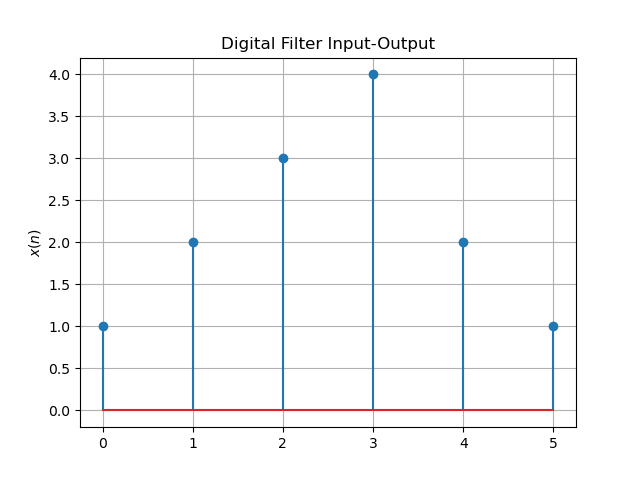
\includegraphics[width=\columnwidth]{./figs/3.1}
	\end{center}
	\captionof{figure}{}
	\label{fig:3.1}	
\end{figure}
\item Let
\begin{multline}
\label{eq:iir_filter}
y(n) + \frac{1}{2}y(n-1) = x(n) + x(n-2), 
\\
 y(n) = 0, n < 0
\end{multline}
Sketch $y(n)$.
\\
\solution The following code yields Fig. \ref{fig:3.2}.
\begin{lstlisting}
wget https://github.com/Pradeep8802/EE3900-Digital-Signal-Processing/blob/main/Assignment1/codes/3.2.py
\end{lstlisting}
\begin{figure}[!ht]
\begin{center}
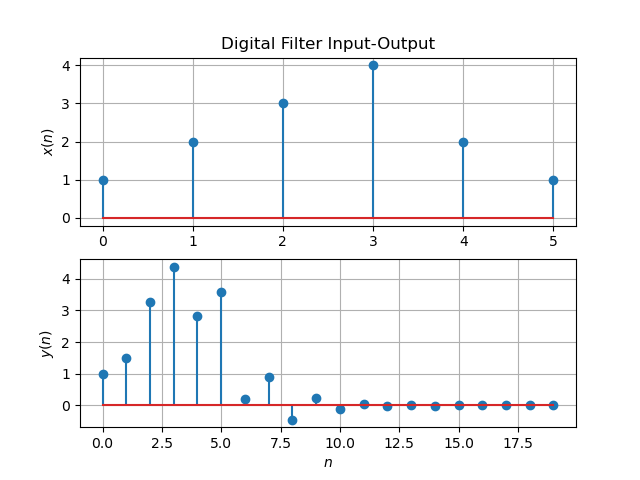
\includegraphics[width=\columnwidth]{./figs/3.2}
\end{center}
\captionof{figure}{}
\label{fig:3.2}	
\end{figure}
\item Repeat the above exercise using a C code.
\solution The following c code is used to find $y(n)$
\begin{lstlisting}
	wget https://github.com/Pradeep8802/EE3900-Digital-Signal-Processing/blob/main/Assignment1/codes/3.3.c
\end{lstlisting}
The following code yields Fig. \ref{fig:3.3}.
\begin{lstlisting}
	wget https://github.com/Pradeep8802/EE3900-Digital-Signal-Processing/blob/main/Assignment1/codes/3.3.py
\end{lstlisting}
\begin{figure}[!ht]
	\begin{center}
		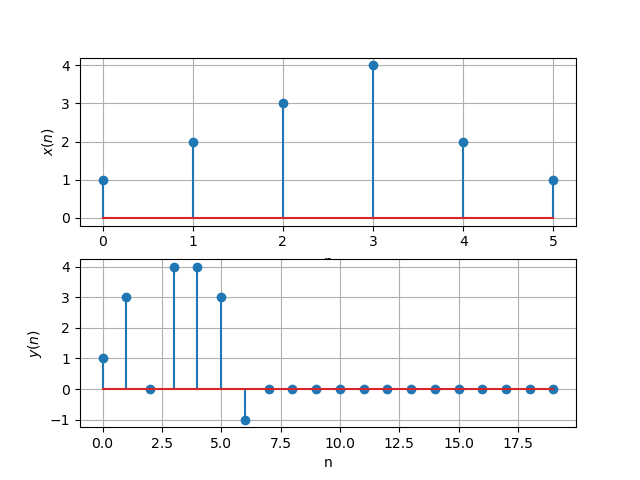
\includegraphics[width=\columnwidth]{./figs/3.3}
	\end{center}
	\captionof{figure}{}
	\label{fig:3.3}	
\end{figure}
\end{enumerate}
\section{$Z$-transform}
\begin{enumerate}[label=\thesection.\arabic*]
\item The $Z$-transform of $x(n)$ is defined as
%
\begin{equation}
\label{eq:z_trans}
X(z)={\mathcal {Z}}\{x(n)\}=\sum _{n=-\infty }^{\infty }x(n)z^{-n}
\end{equation}
%
Show that
\begin{equation}
\label{eq:shift1}
{\mathcal {Z}}\{x(n-1)\} = z^{-1}X(z)
\end{equation}
and find
\begin{equation}
	{\mathcal {Z}}\{x(n-k)\} 
\end{equation}
\solution From \eqref{eq:z_trans},
\begin{align}
{\mathcal {Z}}\{x(n-1)\} &=\sum _{n=-\infty }^{\infty }x(n-1)z^{-n}
\\
&=\sum _{n=-\infty }^{\infty }x(n)z^{-n-1} = z^{-1}\sum _{n=-\infty }^{\infty }x(n)z^{-n}
\end{align}
resulting in \eqref{eq:shift1}. Similarly, it can be shown that
%
\begin{equation}
\label{eq:z_trans_shift}
	{\mathcal {Z}}\{x(n-k)\} = z^{-k}X(z)
\end{equation}



\item Obtain $X(z)$ for $x(n)$ defined in problem 
\ref{def:xn}.
\solution $Z$-transform of x(n),$X(z)$ is given by
\begin{align}
	\mathcal{Z}\{x(n)\}&=\sum_{n=-\infty}^\infty x(n)z^{-n}\\
	&=\sum_{n=0}^5x(n)z^{-n}\\
	&=1+2z^{-1}+3z^{-2}+4z^{-3}+2z^{-4}+z^{-5}
\end{align}


%
%For $x(n) = \cbrak{\underset{\uparrow}{1},2,3,4,2,1}$
%\begin{align}
%	{\mathcal {Z}}\{x(n)\} &=\sum _{n=-\infty }^{\infty }x(n)z^{-n}
%	\\
%	{\mathcal {Z}}\{x(n)\} &=x(0)
%	&=\sum _{n=-\infty }^{\infty }x(n)z^{-n-1} = z^{-1}\sum _{n=-\infty }^{\infty }x(n)z^{-n}
%\end{align}
%\begin{equation}
%	x(n) = \cbrak{\underset{\uparrow}{1},2,3,4,2,1}
%\end{equation}
%
%





\item Find
%
\begin{equation}
H(z) = \frac{Y(z)}{X(z)}
\end{equation}
%
from  \eqref{eq:iir_filter} assuming that the $Z$-transform is a linear operation.
\\
\solution  Applying \eqref{eq:z_trans_shift} in \eqref{eq:iir_filter},
\begin{align}
Y(z) + \frac{1}{2}z^{-1}Y(z) &= X(z)+z^{-2}X(z)
\\
\implies \frac{Y(z)}{X(z)} &= \frac{1 + z^{-2}}{1 + \frac{1}{2}z^{-1}}
\label{eq:freq_resp}
\end{align}
%
\item Find the Z transform of 
\begin{equation}
\delta(n)
=
\begin{cases}
1 & n = 0
\\
0 & \text{otherwise}
\end{cases}
\end{equation}
and show that the $Z$-transform of
\begin{equation}
\label{eq:unit_step}
u(n)
=
\begin{cases}
1 & n \ge 0
\\
0 & \text{otherwise}
\end{cases}
\end{equation}
is
\begin{equation}
U(z) = \frac{1}{1-z^{-1}}, \quad \abs{z} > 1
\end{equation}
\solution The $Z$-transform of $\delta(n)$ is defined as
\begin{align}
	{\mathcal {Z}}\{\delta(n)\}&=\sum _{n=-\infty }^{\infty }\delta(n)z^{-n}\\
	&=\delta(0)z^{-0}\\
	&=1
\end{align}
Hence we can say that
\begin{equation}
\label{eq:z_trans1}
\delta(n) \ztrans 1
\end{equation}
and from \eqref{eq:unit_step},
\begin{align}
U(z) &= \sum _{n= 0}^{\infty}z^{-n}
\\
&=\frac{1}{1-z^{-1}}, \quad \abs{z} > 1
\end{align}
using the fomula for the sum of an infinite geometric progression.
%
\item Show that 
\begin{equation}
\label{eq:anun}
a^nu(n) \ztrans \frac{1}{1-az^{-1}} \quad \abs{z} > \abs{a}
\end{equation}
\solution
\begin{align}
	{\mathcal {Z}}\{a^nu(n)\}&=\sum _{n=-\infty }^{\infty }a^nu(n)z^{-n}\\
	&=\sum _{n=0 }^{\infty }a^nz^{-n}\\
	&=\sum _{n=0 }^{\infty }(z^{-1}a)^{n}\\
	&=\frac{1}{1-az^{-1}}, \quad \abs{z^{-1}a} < 1\\
	&=\frac{1}{1-az^{-1}}, \quad \abs{z} > \abs{a} 
\end{align}
using the fomula for the sum of an infinite geometric progression.
%
\item 
Let
\begin{equation}
H\brak{e^{\j \omega}} = H\brak{z = e^{\j \omega}}.
\end{equation}
Plot $\abs{H\brak{e^{\j \omega}}}$.  Is it periodic? If so, find the period.  $H(e^{\j \omega})$ is
known as the {\em Discret Time Fourier Transform} (DTFT) of $h(n)$.
\\
\solution 
\begin{lstlisting}
wget https://github.com/Pradeep8802/EE3900-Digital-Signal-Processing/blob/main/Assignment1/codes/4.5.py
\end{lstlisting}

$H(e^{jw})$ is given by
\begin{figure}[!ht]
	\centering
	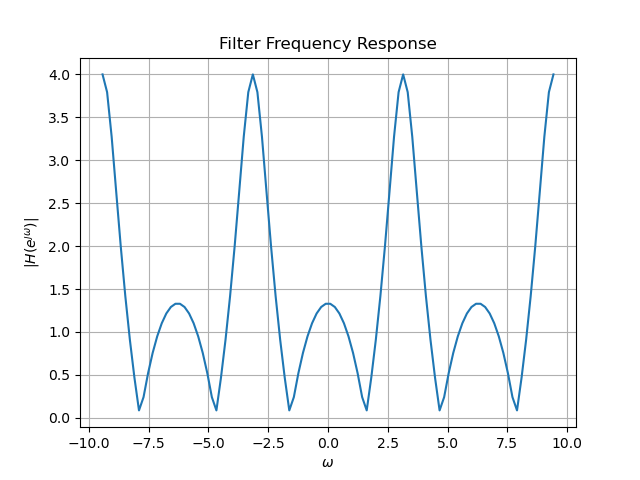
\includegraphics[width=\columnwidth]{./figs/4.5}
	\caption{$\abs{H\brak{e^{\j\omega}}}$}
	\label{fig:4.5}
\end{figure}
\begin{align}
	H(e^{jw})&=\frac{1+(e^{jw})^{-2}}{1+\frac{1}{2}(e^{jw})^{-1}}\\
	&=2\frac{1+\cos(-2\omega)+j\sin(-2\omega)}{2+\cos(-\omega)+j\sin(-\omega)}\\
	&=2\frac{1+\cos(2\omega)-j\sin(2\omega)}{2+\cos(\omega)-j\sin(\omega)}\\
	&=2\frac{2\cos^2(\omega)-2j\sin(\omega)\cos(\omega)}{2+\cos(\omega)-j\sin(\omega)}\\
	&=4\cos(\omega)\frac{\cos(\omega)-j\sin(\omega)}{2+\cos(\omega)-j\sin(\omega)}\\
	&=4|\cos(\omega)| \frac{e^{jw}}{2+e^{jw}}
\end{align}
So,
\begin{align}
	|H(e^{jw})|&=4 |\cos(\omega)| \frac{|e^{jw}|}{|2+e^{jw}|}\\
	&=\frac{|4\cos(\omega)|}{\sqrt{5+4\cos(\omega)}}
\end{align}
The period of $|\cos(\omega)|$ is $\pi$. The period of $5+4\cos(\omega)$ is $2\pi$. Hence $\abs{H\brak{e^{\j\omega}}}$ is periodic with period $2\pi$.( The LCM of the period of $|\cos(\omega)|$ and $5+4\cos(\omega)$ is $2\pi$)
The graph of $\abs{H\brak{e^{\j\omega}}}$ is symmetric with respect to y-axis. It is continuous over $\omega$. The following code plots Fig. \ref{fig:4.5}.

\item Express $h(n)$ in terms of $H\brak{e^{\j \omega}}$.\\
\solution We know that 
\begin{align}
	H(e^{j\omega})=\sum_{k=-\infty}^\infty h(k)e^{-j\omega k}
\end{align}

\begin{align}
	\frac{1}{2\pi}\int_{-\pi}^\pi& H(e^{j\omega})e^{j\omega n}d\omega\\
	&=\frac{1}{2\pi}\int_{-\pi}^\pi \sum_{k=-\infty}^\infty h(k)e^{-j\omega k}e^{j\omega n}d\omega\\
	&=\frac{1}{2\pi} \sum_{k=-\infty}^\infty h(k)\int_{-\pi}^\pi e^{j\omega (n-k)}d\omega\\
\end{align}
case-1:If($n\neq k$)
\begin{align}
	&=\frac{1}{2\pi} \sum_{k\neq n} h(k)\frac{e^{j\omega (n-k)}}{j(n-k)}\Biggr] _{-\pi}^\pi \\
	&=\frac{1}{2\pi} \sum_{k\neq n} h(k)\frac{2\sin(\pi(n-k))}{(n-k)}\\
	&=0
\end{align}
case-2:If($n=k$)
\begin{align}
	&=\frac{1}{2\pi}  h(n)\int_{-\pi}^\pi d\omega\\
	&=h(n)
\end{align}
Hence, we can say,
\begin{align}
	h(n)=\frac{1}{2\pi}\int_{-\pi}^\pi H(e^{j\omega})e^{j\omega n}d\omega 
\end{align}
\end{enumerate}

\section{Impulse Response}
\begin{enumerate}[label=\thesection.\arabic*]
	\item Using long division, 
	find
	\begin{align}
		h(n), \quad n < 5
	\end{align}
	for H(z) in 
	\eqref{eq:freq_resp}.\\
	\solution $H(z)$ is given by
	\begin{align}
		H(z)=\frac{1+z^{-2}}{1+\frac{1}{2}z^{-1}}=\frac{2+2z^{-2}}{2+z^{-1}}
	\end{align}
	\begin{align}
		&2z^{-1}-4\\	
		z^{-1}+2\hspace{2mm}&\overline{\big)\hspace{2mm} 2z^{-2}+2\hspace{15mm}}\\
		& \hspace{2mm} 2z^{-2}+4z^{-1}\\
		&\overline{\hspace{11mm}-4z^{-1}+2\hspace{5mm}}\\
		&\hspace{9mm}-4z^{-1}-8\\ 
		&\overline{\hspace{24mm}10}
	\end{align}
	So,
	\begin{align}
		H(z)&=2z^{-1}-4+\frac{10}{z^{-1}+2}\\
		&=2z^{-1}-4+\frac{5}{\frac{1}{2}z^{-1}+1}\\
		&=2z^{-1}-4+5\sum_{n=0}^\infty \brak{-\frac{z^{-1}}{2}}^{n}\\
		&=1-\frac{1}{2}z^{-1}+5 \times \sum_{n=2}^\infty \brak{-\frac{1}{2}}^{n}z^{-n}
	\end{align}
	So,h(n) will be given by 
	\begin{align}
		h(n)=\begin{cases}
			\label{eq:h_n_def}
			5\times \brak{-\frac{1}{2}}^n  & n\geq 2\\
			\brak{-\frac{1}{2}}^n  &2>n\geq0\\
			0 &n<0
		\end{cases}
	\end{align}
	\item \label{prob:impulse_resp}
	Find an expression for $h(n)$ using $H(z)$, given that 
	%in Problem \ref{eq:ztransab} and \eqref{eq:anun}, given that
	\begin{equation}
		\label{eq:impulse_resp}
		h(n) \ztrans H(z)
	\end{equation}
	and there is a one to one relationship between $h(n)$ and $H(z)$. $h(n)$ is known as the {\em impulse response} of the
	system defined by \eqref{eq:iir_filter}.
	\\
	\solution From \eqref{eq:freq_resp},
	\begin{align}
		H(z) &= \frac{1}{1 + \frac{1}{2}z^{-1}} + \frac{ z^{-2}}{1 + \frac{1}{2}z^{-1}}
		\\
		\implies h(n) &= \brak{-\frac{1}{2}}^{n}u(n) + \brak{-\frac{1}{2}}^{n-2}u(n-2)
	\end{align}
	using \eqref{eq:anun} and \eqref{eq:z_trans_shift}.
	\item Sketch $h(n)$. Is it bounded? Justify theoreti-
	cally.
	\\
	\solution The following code plots Fig. \ref{fig:5.3}.
	\begin{lstlisting}
wget https://github.com/Pradeep8802/EE3900-Digital-Signal-Processing/blob/main/Assignment1/codes/5.3.py
	\end{lstlisting}
	on simplfying we get h(n) as
	\begin{align}
		\begin{cases}
			%\label{eq:h_n_def}
			5\times \brak{-\frac{1}{2}}^n  & n\geq 2\\
			\brak{-\frac{1}{2}}^n  &2>n\geq0\\
			0 &n<0
		\end{cases}
	\end{align}
	\begin{align}
		\because 5\times \brak{-\frac{1}{2}}^n \to 0 \quad	\text{for} \quad n\to \infty 
	\end{align}
	So, we can conclude that h(n) is bounded.
	\begin{figure}[!ht]
		\centering
		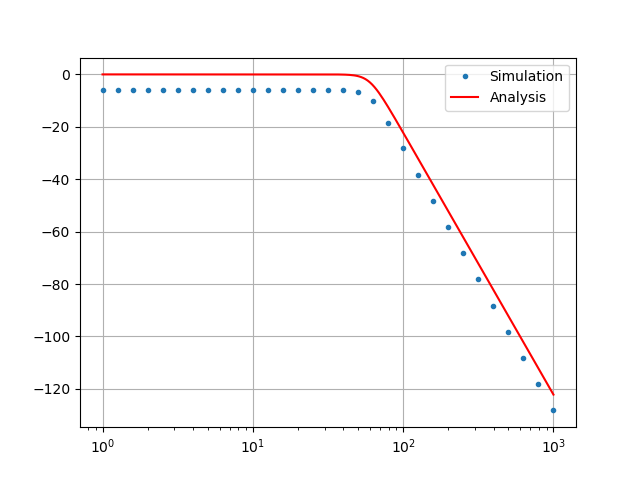
\includegraphics[width=\columnwidth]{./figs/5.3.png}
		\caption{$h(n)$ wrt n}
		\label{fig:5.3}
	\end{figure}
	%
     \item Convergent? Justify using the ratio test.\\
\solution We can say a given real sequence $\cbrak{x_n}$ is convergent if 
\begin{align}
	\lim_{n \rightarrow \infty}\abs{\frac{x_{n+1}}{x_n}} < 1
\end{align}
This is known as Ratio test.\\
In this case the limit will become,
\begin{align}
	\lim_{n \rightarrow \infty}\abs{\frac{h\brak{n+1}}{h\brak{n}}} &= \lim_{n \rightarrow \infty}\abs{\frac{5\brak{\frac{-1}{2}}^{n+1}}{5\brak{\frac{-1}{2}}^{n}}} \\
	&= \lim_{n \rightarrow \infty}\abs{\frac{-1}{2}}\\
	&= \frac{1}{2}
\end{align}
As $\frac{1}{2} < 1$, from root test we can say that $h\brak{n}$ is convergent.
	\item The system with $h(n)$ is defined to be stable if
	\begin{equation}
		\sum_{n=-\infty}^{\infty}h(n) < \infty
	\end{equation}
	Is the system defined by \eqref{eq:iir_filter} stable for the impulse response in \eqref{eq:impulse_resp}?\\
	\solution For system of 3.2 ,$h(n)$ is defined in \eqref{eq:h_n_def} 
	So,
	\begin{align}
		\sum_{n=-\infty}^{\infty}h(n)&=\sum_{n=2}^{\infty}5\times \brak{-\frac{1}{2}}^n+\sum_{n=0}^{1} \brak{-\frac{1}{2}}^n+\sum_{n=-\infty}^{-1}0\\
		&=5\times \frac{1}{6}+\frac{1}{2}\\
		&=\frac{4}{3}
	\end{align}
	Since the sum is finite so the system is stable for impulsive response
	\item Verify the above result using a python code.\\
	\solution The above result is verified using the below python code
		\begin{lstlisting}
wget https://github.com/Pradeep8802/EE3900-Digital-Signal-Processing/tree/main/Assignment1/codes/5.6.py
	\end{lstlisting}
	\item 
	Compute and sketch $h(n)$ using 
	\begin{equation}
		\label{eq:iir_filter_h}
		h(n) + \frac{1}{2}h(n-1) = \delta(n) + \delta(n-2), 
	\end{equation}
	%
	This is the definition of $h(n)$.
	\\
	\solution The following code plots Fig. \ref{fig:h_n_delta}. Note that this is the same as Fig. 
	\ref{fig:3.1}. 
	%
	\begin{lstlisting}
wget https://github.com/Pradeep8802/EE3900-Digital-Signal-Processing/tree/main/Assignment1/codes/5.7.py
	\end{lstlisting}
	\begin{figure}[!ht]
		\centering
		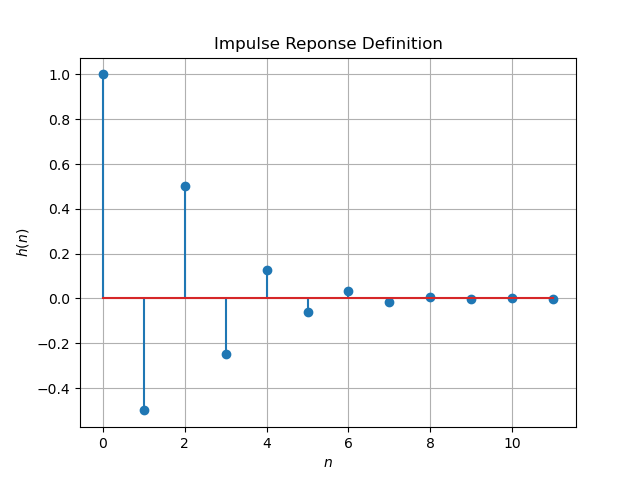
\includegraphics[width=\columnwidth]{./figs/5.7.png}
		\caption{$h(n)$ from the definition}
		\label{fig:h_n_delta}
	\end{figure}
	%
	\item Compute 
	%
	\begin{equation}
		\label{eq:convolution}
		y(n) = x(n)*h(n) = \sum_{k=-\infty}^{\infty}x(k)h(n-k)
	\end{equation}
	%
	Comment. The operation in \eqref{eq:convolution} is known as
	{\em convolution}.
	%
	\\
	\solution The following code plots Fig. \ref{fig:y_n_convo}. Note that this is the same as 
	$y(n)$ in  Fig. 
	\ref{fig:3.1}. 
	\begin{lstlisting}
wget https://github.com/Pradeep8802/EE3900-Digital-Signal-Processing/tree/main/Assignment1/codes/5.4.py
	\end{lstlisting}
	\begin{figure}[!ht]
		\centering
		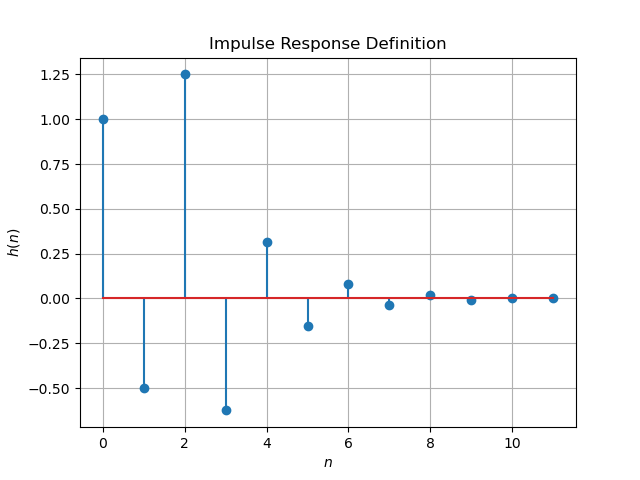
\includegraphics[width=\columnwidth]{./figs/5.4.png}
		\caption{$y(n)$ from the definition of convolution}
		\label{fig:y_n_convo}
	\end{figure}
	  \item Express the above convolution using a Toeplitz matrix.\\
	\solution 
	\begin{figure}
		\centering
		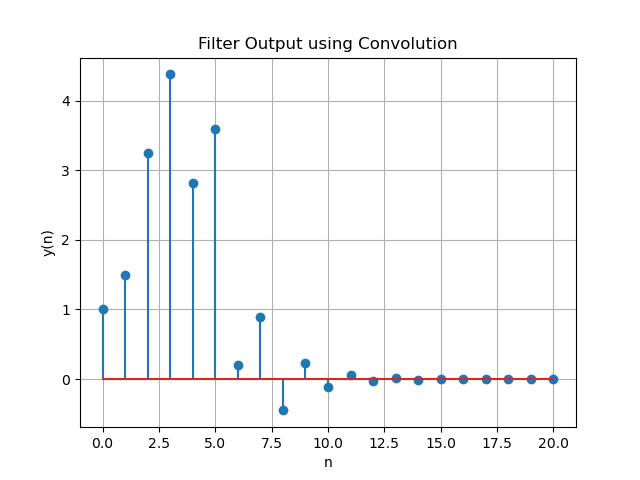
\includegraphics[width = \columnwidth]{figs/5.9.png}
		\caption{Convolution of $x\brak{n}$ and $h\brak{n}$ using toeplitz matrix}
		\label{5.9}
	\end{figure}
	\begin{lstlisting}
wget https://github.com/Pradeep8802/EE3900-Digital-Signal-Processing/tree/main/Assignment1/codes/5.9.py
	\end{lstlisting}

	From $\eqref{eq:convolution}$,we express $y\brak{n}$ as
	\begin{align}
		y\brak{n} &= \sum_{k = -\infty}^{\infty}x\brak{k}h\brak{n-k}
	\end{align}
	To understand how we can use a Toeplitz matrix, we will see what we are doing in $\eqref{eq:convolution}$ 
	\begin{align}
		y\brak{0} &= x\brak{0}h\brak{0}\\
		y\brak{1} &= x\brak{0}h\brak{1} + x\brak{1}h\brak{0}\\
		y\brak{2} &= x\brak{0}h\brak{2} + x\brak{1}h\brak{1} + x\brak{2}h\brak{0}\\
		. \nonumber&\\ 
		.& \nonumber
	\end{align}
	The same thing can be written as,
	\begin{align}
		y\brak{0} &= \myvec{h\brak{0} & 0 & 0 &.\,&.\,&.0}\myvec{x\brak{0}\\x\brak{1}\\x\brak{2}\\ . \\.\\x\brak{5}}\\
		y\brak{1} &= \myvec{h\brak{1} & h\brak{0} & 0 & 0 &.\,&.\,&.0}\myvec{x\brak{0}\\x\brak{1}\\x\brak{2}\\ . \\.\\x\brak{5}}\\
		y\brak{2} &= \myvec{h\brak{2} & h\brak{1} & h\brak{0} & 0& .\,&.0}\myvec{x\brak{0}\\x\brak{1}\\x\brak{2}\\ . \\.\\x\brak{5}}\\
		. & \nonumber \\
		.& \nonumber
	\end{align}
	Using Toeplitz matrix of $h\brak{n}$ we can simplify it as,
	\begin{align}
		y\brak{n} &= \myvec{h\brak{0} & 0 & 0 &.\,&.\,&.\,0 \\
			h\brak{1} & h\brak{0} & 0 & .\,&.\,&.\,0 \\
			h\brak{2} & h\brak{1} & h\brak{0} & .\,&.\,&.\,0 \\
			&&..\\&&..\\ 0 & 0 &  0 &.\,&.\,&.\, h\brak{m-1}}\myvec{x\brak{0}\\x\brak{1}\\x\brak{2}\\ . \\.\\x\brak{5}}\label{eq:5.9}
	\end{align}
	Now from $\eqref{def:xn}$ we will take n 
	\begin{align}
		x\brak{n} &= \myvec{1\\2\\3\\4\\2\\1}
	\end{align}
	And from $\eqref{eq:h_n_def}$ we will take some values of n,
	\begin{align} 
		h\brak{n} &= \myvec{1 \\ -0.5 \\ 1.25 \\. \\ . }
	\end{align}
	Now using $\eqref{eq:5.9}$,
	\begin{align}
		y\brak{n} &= x\brak{n}*h\brak{n}\\
		&= \myvec{1 & 0 & 0 &.\,&.\,&.\,0 \\
			-0.5 & 1 & 0 & .\,&.\,&.\,0 \\
			1.25 & -0.5 & 1 & .\,&.\,&.\,0 \\
			&&..\\&&..\\ 0 & 0 &  0 &.\,&.\,&.\, }\myvec{x\brak{0}\\x\brak{1}\\x\brak{2}\\ . \\.\\x\brak{5}} \\
		&= \myvec{1\\1.5\\3.25\\.\\.\\.}
		\label{eq:topliz}
	\end{align}
The above equation \eqref{eq:topliz} is the convolution of $x(n)$ and $h(n)$
	
	
	
\item Show that
	\begin{equation}
		y(n) =  \sum_{k=-\infty}^{\infty}x(n-k)h(k)
	\end{equation}
\solution From \eqref{eq:convolution}, 
	\begin{align}
		y(n) = \sum_{k=-\infty}^{\infty}x(k)h(n-k)
	\end{align}
	Replacing $n-k$ with $a$,we get
	\begin{align}
		y(n) &= \sum_{n-a=-\infty}^{\infty}x(n-a)h(a)\\
		&=\sum_{-a=-\infty}^{\infty}x(n-a)h(a)\\
		&=\sum_{a=-\infty}^{\infty}x(n-a)h(a)
	\end{align}
\end{enumerate}
%
%%
\section{DFT and FFT}
\begin{enumerate}[label=\thesection.\arabic*]
\item
Compute 
\begin{equation}
X(k) \define \sum _{n=0}^{N-1}x(n) e^{-\j2\pi kn/N}, \quad k = 0,1,\dots, N-1
\end{equation}
and $H(k)$ using $h(n)$.\\
\solution 
Run the following codes to compute $X(k)$ which is plotted in \ref{fig:6.1}.
\begin{lstlisting}
wget https://github.com/Pradeep8802/EE3900-Digital-Signal-Processing/blob/main/Assignment1/codes/6.1.py
\end{lstlisting}
Run the following codes to compute $H(k)$.
\begin{lstlisting}
wget https://github.com/Pradeep8802/EE3900-Digital-Signal-Processing/blob/main/Assignment1/codes/6.1_2.py
\end{lstlisting}
\begin{figure}[!ht]
	\centering
	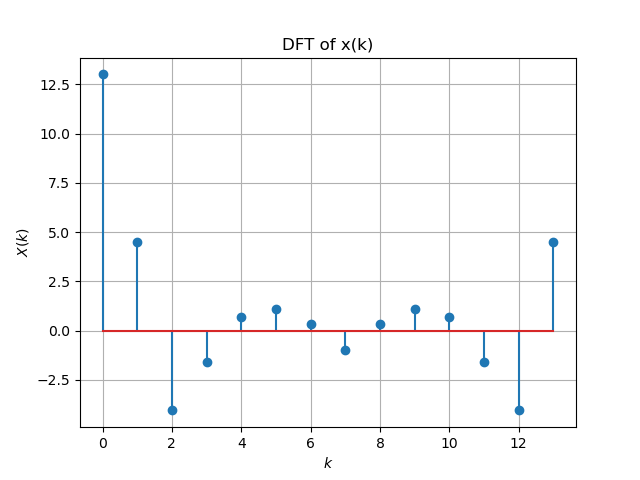
\includegraphics[width=\columnwidth]{./figs/6.1_1.png}
	\caption{DFT of $x(k)$}
	\label{fig:6.1}
\end{figure}

\begin{figure}[!ht]
	\centering
	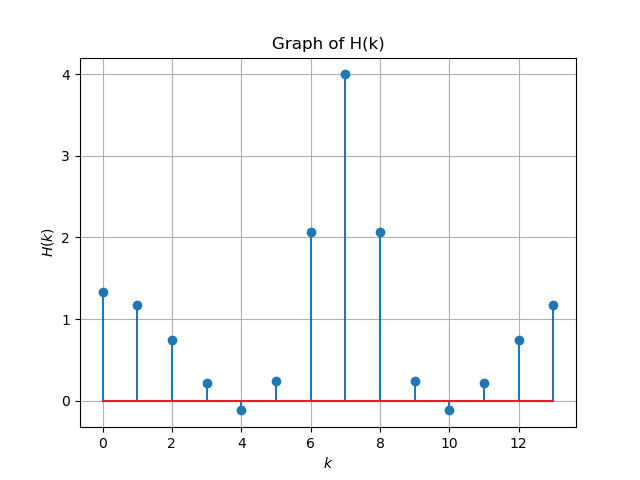
\includegraphics[width=\columnwidth]{./figs/6.1_2.png}
	\caption{$H(n)$}
	\label{fig:6.2}
\end{figure}
\item Compute 
\begin{equation}
Y(k) = X(k)H(k)
\end{equation}
\solution 
Run the following codes to compute $Y(k)$ respectively.
\begin{lstlisting}
wget https://github.com/Pradeep8802/EE3900-Digital-Signal-Processing/blob/main/Assignment1/codes/6.2.py
\end{lstlisting}
\begin{figure}[!ht]
	\centering
	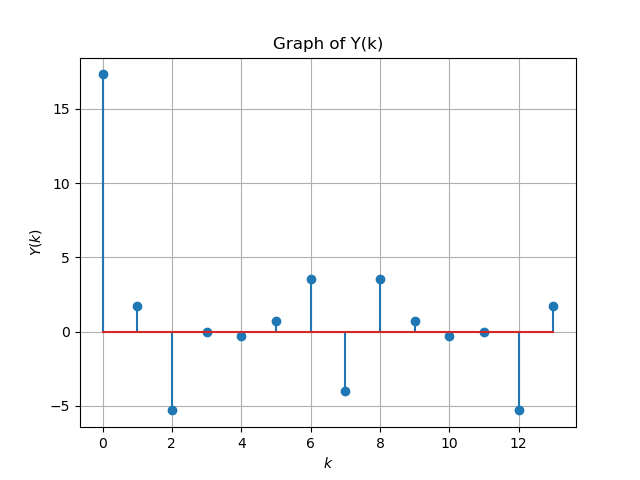
\includegraphics[width=\columnwidth]{./figs/6.2.png}
	\caption{DFT of $xyn)$}
	\label{fig:6.3}
\end{figure}

\item Compute
\begin{equation}
y\brak{n}={\frac {1}{N}}\sum _{k=0}^{N-1}Y\brak{k}\cdot e^{\j 2\pi kn/N},\quad n = 0,1,\dots, N-1
\end{equation}
\\
\solution The following code plots Fig. \ref{fig:6.3}. Note that this is the same as 

$y(n)$ in  Fig. 
\ref{fig:3.1}. 
%
\begin{lstlisting}
wget https://github.com/Pradeep8802/EE3900-Digital-Signal-Processing/blob/main/Assignment1/codes/6.3.py
\end{lstlisting}
\begin{figure}[!ht]
\centering
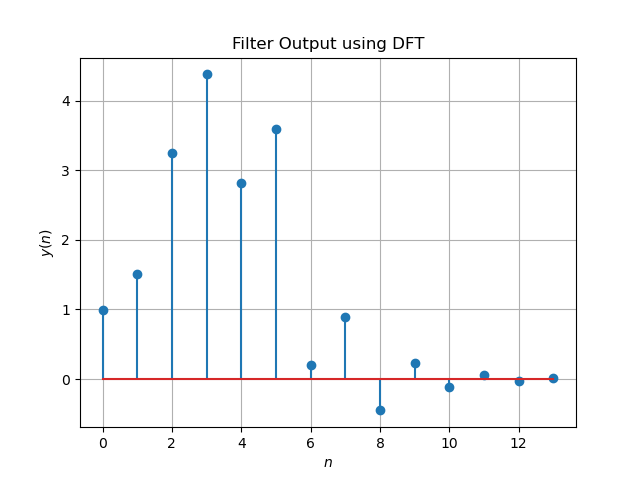
\includegraphics[width=\columnwidth]{./figs/6.3.png}
\caption{$y(n)$}
\label{fig:6.4}
\end{figure}
%
%\item Repeat the previous exercise by computing $X(k), H(k)$ and $y(n)$ through FFT and 
%IFFT.
%\item Wherever possible, express all the above equations as matrix equations.
%\end{enumerate}
%
%\section{Exercises}
%
%Answer the following questions by looking at the python code in Problem \ref{prob:output}.
%\begin{enumerate}[label=\thesection.\arabic*]
%\item
%The command
%\begin{lstlisting}
%	output_signal = signal.lfilter(b, a, input_signal)
%	\end{lstlisting}
%in Problem \ref{prob:output} is executed through the following difference equation
%\begin{equation}
%\label{eq:iir_filter_gen}
% \sum _{m=0}^{M}a\brak{m}y\brak{n-m}=\sum _{k=0}^{N}b\brak{k}x\brak{n-k}
%\end{equation}
%%
%where the input signal is $x(n)$ and the output signal is $y(n)$ with initial values all 0. Replace
%\textbf{signal.filtfilt} with your own routine and verify.
%%
%\item Repeat all the exercises in the previous sections for the above $a$ and $b$.
%
%\item What is the sampling frequency of the input signal?
%\\
%\solution
%Sampling frequency(fs)=44.1kHZ.
%\item
%What is type, order and  cutoff-frequency of the above butterworth filter
%\\
%\solution
%The given butterworth filter is low pass with order=2 and cutoff-frequency=4kHz.
%%
%\item
%Modifying the code with different input parameters and to get the best possible output.
%%

	\item Repeat the previous exercise by computing $X(k), H(k)$ and $y(n)$ through FFT and 
	IFFT.\\
	\solution 
	Run the following code to plot 
	\begin{lstlisting}
wget https://github.com/Pradeep8802/EE3900-Digital-Signal-Processing/blob/main/Assignment1/codes/6.4.py
	\end{lstlisting}
	
\begin{figure}[!ht]
	\centering
	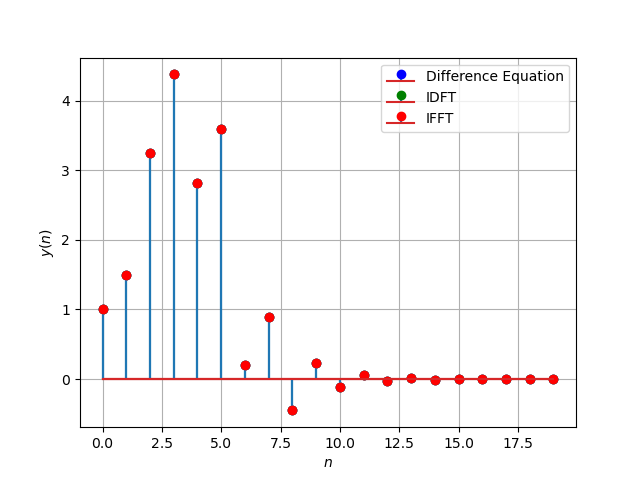
\includegraphics[width=\columnwidth]{./figs/6.4.png}
	\caption{ $y(n)$ }
	% $y(n)$ from the DFT
	\label{fig:6.5}
\end{figure}
%	\begin{figure}[!ht]
%		\centering
%		\includegraphics[width=\columnwidth]{/home/pranav/Desktop/Signal processing/6/fft_ifft}
%		\caption{IFFT}
%		\label{fig:fft_ifft}
%	\end{figure}
%	\item Wherever possible, express all the above equations as matrix equations.
%	\\
%	\solution 
%	\begin{align}
%		\vec{x} &= \myvec{x_0 & x_1	 & \cdots & x_{N-1}}^\top \\
%		\vec{h} &= \myvec{x_0 & x_1	 & \cdots & x_{N-1}}^\top \\
%		\vec{y} &= \vec{x} \circledast \vec{h} \\
%		\myvec{y_1 \\ y_2 \\ \vdots \\ y_{2N - 1}} &= \myvec{
%			h_0 & 0 & 0 & \cdots & 0 \\
%			h_1 & h_0 & 0 & \cdots & 0 \\
%			h_2 & h_1 & h_0 & \cdots & 0 \\
%			\vdots & \vdots & \vdots & \ddots & \vdots \\
%			h_{N-1} & h_{N-2} & h_{N-3} & \cdots & h_0 \\
%			0 & h_{N-1} & h_{N-2} & \cdots & h_1 \\
%			0 & 0 & h_{N-1} & \cdots & h_2 \\
%			\vdots & \vdots & \vdots & \ddots & \vdots \\
%			0 & 0 & 0 & \cdots & h_{N-1}
%		}		
%		\myvec{x_1\\x_2\\ \vdots \\x_N}
%	\end{align}
%	
%	The convolution can be written using a Toeplitz matrix. 
%	
%	Consider the DFT matrix
%	\begin{align}
%		\vec{W} = \myvec{
%			1 & 1 & 1 & 1 & \cdots & 1 \\
%			1 & \omega & \omega^2 & \omega^3 & \cdots & \omega^{N-1} \\
%			1 & \omega^2 & \omega^4 & \omega^6 & \cdots & \omega^{2(N-1)} \\
%			1 & \omega^3 & \omega^6 & \omega^9 & \cdots & \omega^{3(N-1)} \\
%			\vdots & \vdots & \vdots & \vdots & \ddots & \vdots \\ 
%			1 & \omega^{N-1} & \omega^{2(N-1)} & \omega^{3(N-1)} & \cdots & \omega^{(N-1)(N-1)}
%		}
%	\end{align}
%	
%	where $\omega = e^{-\j 2\pi/N}$ is the $N^{\mathrm{th}}$ root of unity
%	
%	Then the discrete Fourier transforms of $\vec{x}$ and $\vec{h}$ are given by
%	\begin{align}
%		\vec{X} &= \vec{W} \vec{x} \\
%		\vec{H} &= \vec{W} \vec{h}
%	\end{align}
%	
%	$\vec{Y}$ is then given by
%	\begin{equation}
%		\vec{Y} = \vec{X} \circ \vec{H}
%	\end{equation}
%	where $\circ$ denotes the Hadamard product (element-wise multiplication)
%	
%	But $\vec{Y}$ is the discrete Fourier transform of the filter output $\vec{y}$
%	\begin{equation}
%		\vec{Y} = \vec{W} \vec{y}
%	\end{equation}
%	Thus,
%	\begin{align}
%		\vec{W} \vec{y} &= \vec{X} \circ \vec{H} \\
%		\implies \vec{y} &= \vec{W}^{-1} \brak{\vec{X} \circ \vec{H}} \\
%		&= \vec{W}^{-1} \brak{\vec{W} \vec{x} \circ \vec{W} \vec{h}}
%	\end{align}
%	This is the inverse discrete Fourier transform of $\vec{Y}$
\end{enumerate}
\section{FFT}	
%\subsection{Definitions}
\begin{enumerate}[label=\arabic*.,ref=\thesection.\theenumi]
	\numberwithin{equation}{section}
	\item The DFT of $x(n)$ is given by
	\begin{align}
		X(k) \triangleq \sum_{n=0}^{N-1} x(n) e^{-j 2 \pi k n / N}, \quad k=0,1, \ldots, N-1
	\end{align}
	\item Let 
	\begin{align}
		W_{N} = e^{-j2\pi/N} 
	\end{align}
	Then the $N$-point {\em DFT matrix} is defined as 
	\begin{align}
		\vec{F}_{N} = \sbrak{W_{N}^{mn}}
	\end{align}
	where $W_{N}^{mn}$ are the elements of $\vec{F}_{N}$.
	\item Let 
	\begin{align}
		\vec{I}_4 = \myvec{\vec{e}_4^{1} &\vec{e}_4^{2} &\vec{e}_4^{3} &\vec{e}_4^{4} }
	\end{align}
	be the $4\times 4$ identity matrix.  Then the 4 point {\em DFT permutation matrix} is defined as 
	\begin{align}
		\vec{P}_4 = \myvec{\vec{e}_4^{1} &\vec{e}_4^{3} &\vec{e}_4^{2} &\vec{e}_4^{4} }
	\end{align}
	\item The 4 point {\em DFT diagonal matrix} is defined as 
	\begin{align}
		\vec{D}_4 = diag\myvec{W_{8}^{0} & W_{8}^{1} & W_{8}^{2} & W_{8}^{3}}
	\end{align}


	\item Show that 
	\begin{equation}
		W_{N}^{2}=W_{N/2}
	\end{equation}
	\solution Given
	\begin{align}
		W_{N} &= e^{-j2\pi/N}\\
	\implies	W_{N}^{2}&=e^{2\brak{-j2\pi/N}}\\
		&=e^{-j2\pi/\brak{N/2}}\\
		&=W_{N/2}
	\end{align}
Therefore, hence proved that ,
\begin{align}
	\label{eq:halving}
	W_N^{2}=W_{N/2}
\end{align}
	\item Show that 
	\begin{equation}
		\vec{F}_{4}=
		\begin{bmatrix}
			\vec{I}_{2} & \vec{D}_{2} \\
			\vec{I}_{2} & -\vec{D}_{2}
		\end{bmatrix}
		\begin{bmatrix}
			\vec{F}_{2} & 0 \\
			0 & \vec{F}_{2}
		\end{bmatrix}
		\vec{P}_{4}
		\label{eq:f4qn}
	\end{equation}
	\solution
	$\vec{I}_2$ is a $2\times 2$ identity matrix, for any $2\times 2$ A, we have 
	\begin{align}
		\vec{I}_2 \vec{A}=\vec{A}\vec{I}_2=\vec{A}
	\end{align}
	Consider
	\begin{align}
		\begin{bmatrix}
			\vec{I}_{2} & \vec{D}_{2} \\
			\vec{I}_{2} & -\vec{D}_{2}
		\end{bmatrix}
		\begin{bmatrix}
			\vec{F}_{2} & 0 \\
			0 & \vec{F}_{2}
		\end{bmatrix}
		&=\begin{bmatrix}
			\vec{F}_{2} & \vec{D}_{2}\vec{F}_{2} \\
			\vec{F}_{2} & -\vec{D}_{2}\vec{F}_{2}
		\end{bmatrix}
	\end{align}
	where
	\begin{align}
		\vec{F}_{2}&=\begin{bmatrix}
			1&1\\1&-1
		\end{bmatrix}\\
		\vec{D}_{2}&=diag(W_4^{0},W_4^{1})
		=\begin{bmatrix}
			1&0\\0&-j
		\end{bmatrix}
	\end{align}
Since $W_4= e^{-j2\pi/4}$\\
	As, \begin{align}
		\vec{P}_4 = \myvec{\vec{e}_4^{1} &\vec{e}_4^{3} &\vec{e}_4^{2} &\vec{e}_4^{4} }
	\end{align}
	\begin{align}
		\label{eq:p4}
	\implies	\vec{P}_{4}&=
		\begin{bmatrix}
			1&0&0&0\\0&0&1&0\\0&1&0&0\\0&0&0&1
		\end{bmatrix}\\
	   \label{eq:F4}
		\vec{F}_{4}&=
		\begin{bmatrix}
			1&1&1&1\\1&-j&-1&j\\1&-1&1&-1\\1&j&-1&-j
		\end{bmatrix}
	\end{align}
\begin{align}
	\vec{D}_{2}\vec{F}_{2}&=
	\begin{bmatrix}
		1&0\\0&-j
	\end{bmatrix}
	\begin{bmatrix}
		1&1\\1&-1
\end{bmatrix}\\
&=\begin{bmatrix}
	1&1\\-j&j
\end{bmatrix}
\end{align}
	\begin{align}
		\begin{bmatrix}
			\vec{F}_{2} & \vec{D}_{2}\vec{F}_{2} \\
			\vec{F}_{2} & -\vec{D}_{2}\vec{F}_{2}
		\end{bmatrix}&=
		\begin{bmatrix}
			1&1&1&1\\1&-1&-j&j\\1&1&-1&-1\\1&-1&j&-j
		\end{bmatrix}
		\label{eq:d2f2}
	\end{align}
	Using \eqref{eq:p4} and \eqref{eq:d2f2} in \eqref{eq:f4qn}
	\begin{align}
		\begin{bmatrix}
			\vec{I}_{2} & \vec{D}_{2} \\
			\vec{I}_{2} & -\vec{D}_{2}
		\end{bmatrix}
		\begin{bmatrix}
			\vec{F}_{2} & 0 \\
			0 & \vec{F}_{2}
		\end{bmatrix}
		\vec{P}_{4}=
		\begin{bmatrix}
			\vec{F}_{2} & \vec{D}_{2}\vec{F}_{2} \\
			\vec{F}_{2} & -\vec{D}_{2}\vec{F}_{2}
		\end{bmatrix}\vec{P}_{4}\\
		=\begin{bmatrix}
			1&1&1&1\\1&-1&-j&j\\1&1&-1&-1\\1&-1&j&-j
		\end{bmatrix}\begin{bmatrix}
			1&0&0&0\\0&0&1&0\\0&1&0&0\\0&0&0&1
		\end{bmatrix}\\
	\label{eq:F4solved}
		=\begin{bmatrix}
			1&1&1&1\\1&-j&-1&j\\1&-1&1&-1\\1&j&-1&-j
		\end{bmatrix}
	\end{align}
The  RHS of the equation \eqref{eq:F4solved} is $\vec{F}_4$, from \eqref{eq:F4}.
	\begin{align}
		\therefore \vec{F}_{4}=
		\begin{bmatrix}
			\vec{I}_{2} & \vec{D}_{2} \\
			\vec{I}_{2} & -\vec{D}_{2}
		\end{bmatrix}
		\begin{bmatrix}
			\vec{F}_{2} & 0 \\
			0 & \vec{F}_{2}
		\end{bmatrix}
		\vec{P}_{4}
	\end{align}
	\item Show that 
	\begin{equation}
		\vec{F}_{N}=
		\begin{bmatrix}
			\vec{I}_{N/2} & \vec{D}_{N/2} \\
			\vec{I}_{N/2} & -\vec{D}_{N/2}
		\end{bmatrix}
		\begin{bmatrix}
			\vec{F}_{N/2} & 0 \\
			0 & \vec{F}_{N/2}
		\end{bmatrix}
		\vec{P}_{N}
	\end{equation}
	\solution \\
	Consider the following properties:
	\begin{align}
		W_N^{k\brak{2n+1}}=W_N^{k}W_{N/2}^{kn}
	\end{align}
	\begin{align}
		\label{eq:periodicity}
		W_N^{k+N/2}=e^{- j 2 \pi \sbrak{k+N/2} / N }=e^{- j 2 \pi k / N }e^{- j \pi}\\
		=-W_N^{k}
	\end{align}
	Consider $X\sbrak{k}$,
	\begin{align}
		X\sbrak{k}&=\sum_{n=0}^{N-1}W_N^{kn} x\sbrak{n} \\
		&=\sum_{n=0}^{N/2-1}\sbrak{x\sbrak{2n}W_N^{k\brak{2n}}+x\sbrak{2n+1}W_N^{k\brak{2n+1}}}
	\end{align}
	$k=0,\cdots,N-1$\\
	which is gathering odd and even terms seperately
	which allows us to write
	\begin{align}
		X\sbrak{k}&=\sum_{n=0}^{N/2-1}x\sbrak{2n}W_{N/2}^{kn}+W_N^k\sum_{n=0}^{N/2-1}x\sbrak{2n+1}W_{N/2}^{kn}\\
		\label{eq:mat1}
		&=Y\sbrak{k}+W_N^k Z\sbrak{k} \,k=0,\cdots,N-1
	\end{align}
	where $Y\sbrak{k}$ and $Z\sbrak{k}$ are DFTs of length N/2 of even numbered sequence $\cbrak{x\sbrak{2n}}$ and of the odd numbered sequence $\cbrak{x\sbrak{2n+1}}$, respectively. Here, we cannot proceed for $k\ge N/2$. So, for $k \ge N/2:$
	\begin{align}
		X\sbrak{k+N/2}&=Y\sbrak{k+N/2}+W_N^{k+N/2} Z\sbrak{k+N/2}
	\end{align}
	Using the periodicity of $Y\sbrak{k}$ and $Z\sbrak{k}$ and \eqref{eq:periodicity},
	\begin{align}
		\label{eq:mat2}
		X\sbrak{k+N/2}&=Y\sbrak{k+N/2}-W_N^{k} Z\sbrak{k}
	\end{align}
	Using \eqref{eq:mat1} and \eqref{eq:mat2}, and linear transformation upon them
	\begin{equation}
		\label{eq:fmat}
		\vec{X}_{N}=
		\begin{bmatrix}
			\vec{I}_{N/2} & \vec{D}_{N/2} \\
			\vec{I}_{N/2} & -\vec{D}_{N/2}
		\end{bmatrix}
		\begin{bmatrix}
			\vec{Y_{N/2}}\\\vec{Z_{N/2}}
		\end{bmatrix}
	\end{equation}
	where $\vec{I_{N/2}}$ is a unit matrix and $\vec{D_{N/2}}$ is a diagonal matrix with elements as $\cbrak{W_N^{k},k=0,\cdots,N/2-1}$, both of dimension $N/2 \times N/2$ .Whereas \\
	$\vec{Y_N/2}=$ DFT of even terms of $\vec{X_N}=\vec{F_{N/2}x_{even}}$\\
	$\vec{Z_N/2}=$ DFT of odd terms of $\vec{X_N}=\vec{F_{N/2}x_{odd}}$\\
	which gets us to \\
	\begin{align}
		\begin{bmatrix}
			\vec{Y_{N/2}}\\\vec{Z_{N/2}}
		\end{bmatrix}&=
		\begin{bmatrix}
			\vec{F}_{N/2} & 0 \\
			0 & \vec{F}_{N/2}
		\end{bmatrix}\vec{x}
	\end{align}
	which is permuting into combinations of even and odd terms of a sequence.As we have permuted it into odd and even parts, we have to reverse this process. So, a permutation matrix is multiplied.
	\begin{align}
		\begin{bmatrix}
			\vec{Y_{N/2}}\\\vec{Z_{N/2}}
		\end{bmatrix}&=
		\begin{bmatrix}
			\vec{F}_{N/2} & 0 \\
			0 & \vec{F}_{N/2}
		\end{bmatrix}\vec{P_N}\vec{x}
	\end{align}
	Replacing in \eqref{eq:fmat},
	\begin{equation}
		\vec{X}_{N}=
		\begin{bmatrix}
			\vec{I}_{N/2} & \vec{D}_{N/2} \\
			\vec{I}_{N/2} & -\vec{D}_{N/2}
		\end{bmatrix}
		\begin{bmatrix}
			\vec{F}_{N/2} & 0 \\
			0 & \vec{F}_{N/2}
		\end{bmatrix}\vec{P_N}\vec{x}
	\end{equation}
	As $\vec{X_N}=\vec{F_N}\vec{x}$,
	\begin{align}
		\vec{F_N}\vec{x}=
		\begin{bmatrix}
			\vec{I}_{N/2} & \vec{D}_{N/2} \\
			\vec{I}_{N/2} & -\vec{D}_{N/2}
		\end{bmatrix}
		\begin{bmatrix}
			\vec{F}_{N/2} & 0 \\
			0 & \vec{F}_{N/2}
		\end{bmatrix}\vec{P_N}\vec{x}
	\end{align}
	Applying $\vec{x^{-1}}$,
	\begin{align}
		\label{eq:final}
		\vec{F}_{N}=
		\begin{bmatrix}
			\vec{I}_{N/2} & \vec{D}_{N/2} \\
			\vec{I}_{N/2} & -\vec{D}_{N/2}
		\end{bmatrix}
		\begin{bmatrix}
			\vec{F}_{N/2} & 0 \\
			0 & \vec{F}_{N/2}
		\end{bmatrix}
		\vec{P}_{N}
	\end{align}
	\item Find 
	\begin{align}
		\vec{P}_4 \vec{x}
	\end{align}
	\solution From \eqref{eq:p4},
	\begin{align}
		\vec{P}_4&=\begin{bmatrix}
			1&0&0&0\\0&0&1&0\\0&1&0&0\\0&0&0&1
		\end{bmatrix}\\
		\vec{x}&=\myvec{1\\2\\3\\4\\2\\1}
	\end{align}
	After proper zero padding of $\vec{P}_4$,
	\begin{align}
		\vec{P}_4&=\begin{bmatrix}
			1&0&0&0&0&0\\0&0&1&0&0&0\\0&1&0&0&0&0\\0&0&0&1&0&0\\0&0&0&0&0&0\\0&0&0&0&0&0
		\end{bmatrix}\\
		\vec{P}_4 \vec{x}&=\begin{bmatrix}
			1&0&0&0&0&0\\0&0&1&0&0&0\\0&1&0&0&0&0\\0&0&0&1&0&0\\0&0&0&0&0&0\\0&0&0&0&0&0
		\end{bmatrix}\myvec{1\\2\\3\\4\\2\\1}\\
		&=\myvec{1\\3\\2\\4\\0\\0}
	\end{align}
	\item Show that 
	\begin{align}
		\label{eq:dft-mat-def}
		\vec{X} = \vec{F}_N \vec{x}
	\end{align}
	where $\vec{x}, \vec{X}$ are the vector representations of $x(n), X(k)$ respectively.\\
	\solution Given $\vec{x}, \vec{X}$ are the vector representations of $x(n), X(k)$ respectively.
	\begin{align}
		\vec{x}&=\begin{bmatrix}
			x(0)\\x(1)\\\vdots\\ x(N-1)
		\end{bmatrix}\\
		\vec{X}&=\begin{bmatrix}
			X(0)\\X(1)\\ \vdots\\ X(N-1)
		\end{bmatrix}\\
		\vec{F}_N &=\begin{bmatrix}
			1&1&1&\cdots&1\\1&W_N&W^2_N&\cdots&W_N^{(N-1)}\\1&W_N^2&W_N^4&\cdots&W^{2(N-1)}_N\\\vdots&\vdots&\vdots&\ddots&\vdots\\1&W_N^{N-1}&W_N^{2(N-1)}&\cdots&W_N^{(N-1)(N-1)}
		\end{bmatrix}
	\end{align}
	As \begin{align} 
		X(k)&=\sum_{n=0}^{N-1} x(n) e^{-j 2 \pi k n /N}
	\end{align}
 Here, we have,
 \begin{align}
 X(0)&=	\sum_{n=0}^{N-1} x(n) e^{0}\\
 &=\sum_{n=0}^{N-1} x(n)\\
 X(1)&=	\sum_{n=0}^{N-1} x(n) e^{-j 2 \pi n /N}\\
 &=\sum_{n=0}^{N-1} x(n) W_N^{n} \\
 \vdots\\
 X(N-1)&=\sum_{n=0}^{N-1} x(n) e^{-j 2 \pi (N-1) n /N}\\
 &=\sum_{n=0}^{N-1} x(n) W_N^{n \times (N-1)} 
 \end{align}
Representing the above equations in matrix form as matrix multiplication, we get, 
	\begin{align}
		\begin{bmatrix}
			X(0)\\X(1)\\ \vdots\\ X(N-1)
		\end{bmatrix}
		&=\begin{bmatrix}
			1&1&\cdots&1\\1&W_N&\cdots&W_N^{(N-1)}\\1&W_N^2&\cdots\\\vdots&\vdots&\ddots&\vdots\\1&W_N^{N-1}&\cdots&W_N^{(N-1)(N-1)}
		\end{bmatrix}\begin{bmatrix}
			x(0)\\x(1)\\\vdots\\ x(N-1)
		\end{bmatrix}\\
		\therefore \vec{X} = \vec{F}_N \vec{x}
	\end{align}
%	\begin{align}
%		\begin{bmatrix}
%			X(0)\\X(1)\\ \vdots\\ X(N-1)
%		\end{bmatrix}
%		&=\begin{bmatrix}
%			1&1&1&\cdots&1\\1&W_N&W^2_N&\cdots&W_N^{(N-1)}\\1&W_N^2&W_N^4&\cdots&W^{2(N-1)}_N\\\vdots&\vdots&\vdots&\ddots&\vdots\\1&W_N^{N-1}&W_N^{2(N-1)}&\cdots&W_N^{(N-1)(N-1)}
%		\end{bmatrix}\begin{bmatrix}
%			x(0)\\x(1)\\\vdots\\ x(N-1)
%		\end{bmatrix}\\
%		\therefore \vec{X} = \vec{F}_N \vec{x}
%	\end{align}
	\item Derive the following Step-by-step visualisation  of
	8-point FFTs into 4-point FFTs and so on
	\begin{equation}
		\begin{bmatrix}
			X(0) \\ 
			X(1) \\ 
			X(2) \\ 
			X(3)
		\end{bmatrix}
		=
		\begin{bmatrix}
			X_{1}(0) \\ 
			X_{1}(1)\\ 
			X_{1}(2)\\
			X_{1}(3)\\
		\end{bmatrix}
		+
		\begin{bmatrix}
			W^{0}_{8} & 0 & 0 & 0\\
			0 & W^{1}_{8} & 0 & 0\\
			0 & 0 & W^{2}_{8} & 0\\
			0 & 0 & 0 & W^{3}_{8}
		\end{bmatrix}
		\begin{bmatrix}
			X_{2}(0) \\ 
			X_{2}(1) \\ 
			X_{2}(2) \\
			X_{2}(3)
		\end{bmatrix}
	\end{equation}
	\begin{equation}
		\begin{bmatrix}
			X(4) \\ 
			X(5) \\ 
			X(6) \\ 
			X(7)
		\end{bmatrix}
		=
		\begin{bmatrix}
			X_{1}(0) \\ 
			X_{1}(1)\\ 
			X_{1}(2)\\
			X_{1}(3)\\
		\end{bmatrix}
		-
		\begin{bmatrix}
			W^{0}_{8} & 0 & 0 & 0\\
			0 & W^{1}_{8} & 0 & 0\\
			0 & 0 & W^{2}_{8} & 0\\
			0 & 0 & 0 & W^{3}_{8}
		\end{bmatrix}
		\begin{bmatrix}
			X_{2}(0) \\ 
			X_{2}(1) \\ 
			X_{2}(2) \\
			X_{2}(3)
		\end{bmatrix}
	\end{equation}
	4-point FFTs into 2-point FFTs
	\begin{equation}
		\begin{bmatrix}
			X_{1}(0) \\ 
			X_{1}(1)\\ 
		\end{bmatrix}
		=
		\begin{bmatrix}
			X_{3}(0) \\ 
			X_{3}(1)\\ 
		\end{bmatrix}
		+
		\begin{bmatrix}
			W^{0}_{4} & 0\\
			0 & W^{1}_{4}
		\end{bmatrix}
		\begin{bmatrix}
			X_{4}(0) \\ 
			X_{4}(1) \\ 
		\end{bmatrix}
	\end{equation}
	\begin{equation}
		\begin{bmatrix}
			X_{1}(2) \\ 
			X_{1}(3)\\ 
		\end{bmatrix}
		=
		\begin{bmatrix}
			X_{3}(0) \\ 
			X_{3}(1)\\ 
		\end{bmatrix}
		-
		\begin{bmatrix}
			W^{0}_{4} & 0\\
			0 & W^{1}_{4}
		\end{bmatrix}
		\begin{bmatrix}
			X_{4}(0) \\ 
			X_{4}(1) \\ 
		\end{bmatrix}
	\end{equation}
	\begin{equation}
		\begin{bmatrix}
			X_{2}(0) \\ 
			X_{2}(1)\\ 
		\end{bmatrix}
		=
		\begin{bmatrix}
			X_{5}(0) \\ 
			X_{5}(1)\\ 
		\end{bmatrix}
		+
		\begin{bmatrix}
			W^{0}_{4} & 0\\
			0 & W^{1}_{4}
		\end{bmatrix}
		\begin{bmatrix}
			X_{6}(0) \\ 
			X_{6}(1) \\ 
		\end{bmatrix}
	\end{equation}
	\begin{equation}
		\begin{bmatrix}
			X_{2}(2) \\ 
			X_{2}(3)\\ 
		\end{bmatrix}
		=
		\begin{bmatrix}
			X_{5}(0) \\ 
			X_{5}(1)\\ 
		\end{bmatrix}
		-
		\begin{bmatrix}
			W^{0}_{4} & 0\\
			0 & W^{1}_{4}
		\end{bmatrix}
		\begin{bmatrix}
			X_{6}(0) \\ 
			X_{6}(1) \\ 
		\end{bmatrix}
	\end{equation}
	\begin{equation}
		P_{8}
		\begin{bmatrix}
			x(0) \\ 
			x(1) \\ 
			x(2) \\ 
			x(3) \\ 
			x(4) \\ 
			x(5) \\
			x(6) \\
			x(7)
		\end{bmatrix}
		= 
		\begin{bmatrix}
			x(0) \\ 
			x(2) \\ 
			x(4) \\ 
			x(6) \\
			x(1) \\ 
			x(3) \\ 
			x(5) \\
			x(7)
		\end{bmatrix}
	\end{equation}
	\begin{equation}
		P_{4}
		\begin{bmatrix}
			x(0) \\ 
			x(2) \\ 
			x(4) \\ 
			x(6) \\
		\end{bmatrix}
		= 
		\begin{bmatrix}
			x(0) \\ 
			x(4) \\ 
			x(2) \\
			x(6)
		\end{bmatrix}
	\end{equation}
	\begin{equation}
		P_{4}
		\begin{bmatrix}
			x(1) \\ 
			x(3) \\ 
			x(5) \\
			x(7)
		\end{bmatrix}
		= 
		\begin{bmatrix}
			x(1) \\ 
			x(5) \\ 
			x(3) \\ 
			x(7) \\
		\end{bmatrix}
	\end{equation}
	Therefore,
	\begin{equation}
		\begin{bmatrix}
			X_{3}(0) \\ 
			X_{3}(1)\\ 
		\end{bmatrix}
		= F_{2}
		\begin{bmatrix}
			x(0) \\ 
			x(4) \\ 
		\end{bmatrix}
	\end{equation}
	\begin{equation}
		\begin{bmatrix}
			X_{4}(0) \\ 
			X_{4}(1)\\ 
		\end{bmatrix}
		= F_{2}
		\begin{bmatrix}
			x(2) \\ 
			x(6) \\ 
		\end{bmatrix}
	\end{equation}
	\begin{equation}
		\begin{bmatrix}
			X_{5}(0) \\ 
			X_{5}(1)\\ 
		\end{bmatrix}
		= F_{2}
		\begin{bmatrix}
			x(1) \\ 
			x(5) \\ 
		\end{bmatrix}
	\end{equation}
	\begin{equation}
		\begin{bmatrix}
			X_{6}(0) \\ 
			X_{6}(1)\\ 
		\end{bmatrix}
		= F_{2}
		\begin{bmatrix}
			x(3) \\ 
			x(7) \\ 
		\end{bmatrix}
	\end{equation}
	\item For 
	\begin{align}
		\vec{x} = \myvec{1\\2\\3\\4\\2\\1}
		\label{eq:equation1}
	\end{align}
	compte the DFT  
	using 
	\eqref{eq:dft-mat-def}\\
	\solution \begin{align}
		\vec{F}_6&=\begin{bmatrix}
			1&1&1&1&1&1\\1&e^{-j \pi/3 }&e^{-j 2 \pi/3 }&e^{-j \pi }&e^{-j 4 \pi/3 }&e^{-j 5 \pi/3 }\\1&e^{-j 2 \pi/3 }&e^{-j 4 \pi/3 }&e^{-j 2 \pi }&e^{-j 8\pi/3 }&e^{-j 10 \pi/3 }\\1&e^{-j \pi }&e^{-j 2 \pi }&e^{-j 3 \pi }&e^{-j 4 \pi }&e^{-j 5 \pi }\\1&e^{-j 4 \pi/3 }&e^{-j 8 \pi/3 }&e^{-j 4 \pi }&e^{-j 16 \pi/3 }&e^{-j 20 \pi/3 }\\1&e^{-j 5 \pi/3 }&e^{-j 10 \pi/3 }&e^{-j 5 \pi }&e^{-j 20 \pi/3 }&e^{-j 25 \pi/3 }
		\end{bmatrix}
	\end{align}
	Using \eqref{eq:equation1},
	\begin{align}
		\vec{X}&=\vec{F}_6\vec{x}
	\end{align}
	\begin{align}
		\vec{X}=\begin{bmatrix}
			1&1&1&1&1&1\\1&e^{-j \pi/3 }&e^{-j 2 \pi/3 }&e^{-j \pi }&e^{-j 4 \pi/3 }&e^{-j 5 \pi/3 }\\1&e^{-j 2 \pi/3 }&e^{-j 4 \pi/3 }&e^{-j 2 \pi }&e^{-j 8\pi/3 }&e^{-j 10 \pi/3 }\\1&e^{-j \pi }&e^{-j 2 \pi }&e^{-j 3 \pi }&e^{-j 4 \pi }&e^{-j 5 \pi }\\1&e^{-j 4 \pi/3 }&e^{-j 8 \pi/3 }&e^{-j 4 \pi }&e^{-j 16 \pi/3 }&e^{-j 20 \pi/3 }\\1&e^{-j 5 \pi/3 }&e^{-j 10 \pi/3 }&e^{-j 5 \pi }&e^{-j 20 \pi/3 }&e^{-j 25 \pi/3 }
		\end{bmatrix} \myvec{1\\2\\3\\4\\2\\1}
	\end{align}
	\begin{align}
		\implies X=\begin{bmatrix}
			13\\-4-\sqrt{3}j\\1\\-1\\1\\-4+\sqrt{3}j
		\end{bmatrix}
	\end{align}
	\item Repeat the above exercise using the FFT
	after zero padding $\vec{x}$.\\
	\solution After padding, $\vec{x}$ becomes an $8 \times 1$ matrix, as shown below
	\begin{align}
		\vec{x}=\myvec{1\\2\\3\\4\\2\\1\\0\\0}
	\end{align}
	Using \eqref{eq:final},
	\begin{align}
		\vec{F}_{8}=
		\begin{bmatrix}
			\vec{I}_{4} & \vec{D}_{4} \\
			\vec{I}_{4} & -\vec{D}_{4}
		\end{bmatrix}
		\begin{bmatrix}
			\vec{F}_{4} & 0 \\
			0 & \vec{F}_{4}
		\end{bmatrix}
		\vec{P}_{8}\\
		\vec{F}_{4}=
		\begin{bmatrix}
			\vec{I}_{2} & \vec{D}_{2} \\
			\vec{I}_{2} & -\vec{D}_{2}
		\end{bmatrix}
		\begin{bmatrix}
			\vec{F}_{2} & 0 \\
			0 & \vec{F}_{2}
		\end{bmatrix}
		\vec{P}_{4}\\
		\vec{F}_{2}=
		\begin{bmatrix}
			\vec{I}_{1} & \vec{D}_{1} \\
			\vec{I}_{1} & -\vec{D}_{1}
		\end{bmatrix}
		\begin{bmatrix}
			\vec{F}_{1} & 0 \\
			0 & \vec{F}_{1}
		\end{bmatrix}
		\vec{P}_{2}\\
		\end{align}
	As $\vec{F_1}=\sbrak{W_1^{0}}$, we have
	\begin{align}
		\vec{F_1}&=\sbrak{1}
	\end{align}
	Value of $\vec{F_2}$ is,
	\begin{align}
		\vec{F_2}&=\begin{bmatrix}
			\vec{F}_{1} & \vec{D_1F_1} \\
			\vec{F}_{1} & -\vec{D_1F_1}
		\end{bmatrix}\vec{P_2}\\
		&=\begin{bmatrix}1&1\\1&-1\end{bmatrix}
	\end{align}
	value of $\vec{F_4}$ is,
	\begin{align}
		\vec{D}_{2}=diag(W_4^0,W_4^1)\\
		=diag(1,-j)\\					
		=\begin{bmatrix}
			1&0\\0&-j
		\end{bmatrix}\\
		\vec{D_2F_2}=\begin{bmatrix}
			1&0\\0&-j
		\end{bmatrix}\begin{bmatrix}
			1&1\\1&-1
		\end{bmatrix}\\
		=\begin{bmatrix}
			1&1\\-j&j
		\end{bmatrix}\\
		\vec{F_4}=\begin{bmatrix}
			\vec{F}_{2} & \vec{D_2F_2} \\
			\vec{F}_{2} & -\vec{D_2F_2}
		\end{bmatrix}\vec{P_4}\\
		\vec{F_4}=\begin{bmatrix}
			1&0&1&1\\0&1&-j&j\\1&0&-1&-1\\0&1&j&-j
		\end{bmatrix}\begin{bmatrix}
			1&0&0&0\\0&0&1&0\\0&1&0&0\\0&0&0&1
		\end{bmatrix}\\
		=\begin{bmatrix}
			1&1&0&1\\0&-j&1&j\\1&-1&0&j\\0&j&1&-j
		\end{bmatrix}
	\end{align}
	value of $\vec{F_8}$ is,
	\begin{align}
		\vec{D_4}=diag\brak{1,W_8,W_8^2,W_8^3}\\
		=\begin{bmatrix}
			1&0&0&0\\0&\frac{1-j}{\sqrt{2}}&0&0\\0&0&-1&0\\0&0&0&\frac{-1-j}{\sqrt{2}}
		\end{bmatrix}\\
		\vec{D_4F_4}=\begin{bmatrix}
			1&0&0&0\\0&\frac{1-j}{\sqrt{2}}&0&0\\0&0&-1&0\\0&0&0&\frac{-1-j}{\sqrt{2}}
		\end{bmatrix}\begin{bmatrix}
			1&1&0&1\\0&-j&1&j\\1&-1&0&j\\0&j&1&-j
		\end{bmatrix}\\
		=\begin{bmatrix}
			1&1&0&1\\0&\frac{-1-j}{\sqrt{2}}&\frac{1-j}{\sqrt{2}}&\frac{1+j}{\sqrt{2}}\\-1&1&0&-j\\0&\frac{1-j}{\sqrt{2}}&\frac{-1-j}{\sqrt{2}}&\frac{-1+j}{\sqrt{2}}
		\end{bmatrix}
	\end{align}
	$F_8=\vec{ABP_8}$ where
	\begin{align}
		\vec{A}=\begin{bmatrix}
			1&0&0&0&1&0&0&0\\0&1&0&0&0&\frac{-1-j}{\sqrt{2}}&\frac{1-j}{\sqrt{2}}&\frac{1+j}{\sqrt{2}}\\0&0&1&0&-1&1&0&-j\\0&0&0&1&0&\frac{1-j}{\sqrt{2}}&\frac{-1-j}{\sqrt{2}}&\frac{-1+j}{\sqrt{2}}\\1&0&0&0&-1&0&0&0\\0&1&0&0&0&\frac{1+j}{\sqrt{2}}&\frac{-1+j}{\sqrt{2}}&\frac{-1-j}{\sqrt{2}}\\0&0&1&0&1&-1&0&j\\0&0&0&1&0&\frac{-1+j}{\sqrt{2}}&\frac{1+j}{\sqrt{2}}&\frac{1-j}{\sqrt{2}}
		\end{bmatrix}\\ \vec{B}=\begin{bmatrix}
			1&1&0&1&0&0&0&0\\0&-j&1&j&0&0&0&0\\1&-1&0&j&0&0&0&0\\0&j&1&-j&0&0&0&0\\0&0&0&0&-1&-1&0&-1\\0&0&0&0&0&j&-1&j\\0&0&0&0&-1&1&0&-j\\0&0&0&0&0&-j&-1&j
		\end{bmatrix}\\
		\vec{F_8}=\
	\end{align}
	And $\vec{P_8}$ is a permutation matrix.
	\begin{align}
		\vec{X}=\begin{bmatrix}
			13\\-4-8j\\j\\ 2-2j\\ -1\\ 2+2j\\ -j\\ -4+8j
		\end{bmatrix}
	\end{align}
	\item Write a C program to compute the 8-point FFT.
	\solution 
	\begin{lstlisting}
wget  https://github.com/Pradeep8802/EE3900-Digital-Signal-Processing/blob/main/Assignment1/codes/7_13.py
	\end{lstlisting}
	
	%\begin{lstlisting} 
	%	wget https://github.com/LokeshBadisa/EE3900-Linear-Systems-and-Signal-Processing/blob/main/codes/7.9.c
	%	gcc 7.9.c -lm
	%\end{lstlisting}
\end{enumerate}
%\section{Exercises}
%Answer the following questions by looking at the python code in Problem \ref{prob:output}
%
%\begin{enumerate}[label=\thesection.\arabic*]
%	\item The command
%	\begin{lstlisting}
%		output_signal = signal.lfilter(b, a, input_signal)
%	\end{lstlisting}
%	in Problem \ref{prob:output} is executed through the following difference equation
%	\begin{equation}
%		\label{eq:iir_filter_gen}
%		\sum _{m=0}^{M}a\brak{m}y\brak{n-m}=\sum _{k=0}^{N}b\brak{k}x\brak{n-k}
%	\end{equation}
%	where the input signal is $x(n)$ and the output signal is $y(n)$ with initial values all 0. Replace \textbf{signal.filtfilt} with your own routine and verify.
%	
%	\solution On taking the $Z$-transform on both sides of the difference equation
%	\begin{align}
%		\sum _{m=0}^{M}a\brak{m} z^{-m} Y(z) &= \sum _{k=0}^{N}b\brak{k} z^{-k} X(z) \\
%		\implies H(z) = \frac{Y(z)}{X(z)} &= \frac{\sum _{k=0}^{N}b\brak{k} z^{-k}}{\sum _{m=0}^{M}a\brak{m} z^{-m	}}
%	\end{align}
%	
%	For obtaining the discrete Fourier transform, put $z = \j \frac{2\pi i}{I}$ where $I$ is the length of the input signal and $i = 0, 1, \ldots, I-1$
%	
%	Download the following Python code that does the above
%	\begin{lstlisting}
%		wget https://github.com/LokeshBadisa/EE3900-Linear-Systems-and-Signal-Processing/blob/main/codes/7.1.py
%	\end{lstlisting}
%	
%	\item Repeat all the exercises in the previous sections for the above $a$ and $b$
%	
%	\solution The polynomial coefficients obtained are
%	\begin{align}
%		\vec{a} = \myvec{1.000 \\ -2.519 \\ 2.561 \\ -1.206 \\ 0.220} \qquad
%		\vec{b} = \myvec{0.003 \\ 0.014 \\ 0.021 \\ 0.014 \\ 0.003}
%	\end{align}
%	
%	The difference equation is then given by
%	\begin{equation}
%		\vec{a}^\top \vec{y} = \vec{b}^\top \vec{x} 
%	\end{equation}
%	
%	where
%	\begin{align}
%		\vec{y} = \myvec{y(n) \\ y(n-1) \\ y(n-2) \\ y(n-3) \\ y(n-4)} \qquad
%		\vec{x} = \myvec{x(n) \\ x(n-1) \\ x(n-2) \\ x(n-3) \\ x(n-4)}
%	\end{align}
%	
%	Download the following Python code
%	\begin{lstlisting}
%		wget https://github.com/LokeshBadisa/EE3900-Linear-Systems-and-Signal-Processing/blob/main/codes/7.2.py
%	\end{lstlisting}
%	
%	\begin{figure}[!ht]
%		\centering
%		\includegraphics[width=\columnwidth]{./figs/7.2.1.png}
%		\caption{Plot of $y(n)$}
%		\label{fig-7.2.1}	
%	\end{figure}
%	
%	\begin{figure}[!ht]
%		\centering
%		\includegraphics[width=\columnwidth]{./figs/7.2.2.png}
%		\caption{Plot of $\abs{H(e^{\j\omega})}$}
%		\label{fig-7.2.2}	
%	\end{figure}
%	
%	\begin{figure}[!ht]
%		\centering
%		\includegraphics[width=\columnwidth]{./figs/7.2.3.png}
%		\caption{Plot of $h(n)$}
%		\label{fig-7.2.3}	
%	\end{figure}
%	
%	\item What is the sampling frequency of the input signal?
%	
%	\solution The sampling frequency of the input signal is \SI{44100}{\hertz} = \SI{44.1}{\kilo\hertz}
%	
%	\item What is the type, order and cutoff frequency of the above Butterworth filter?
%	
%	\solution 
%	
%	Type: low-pass
%	
%	Order: 4
%	
%	Cutoff frequency: \SI{4000}{\hertz} = \SI{4}{\kilo\hertz}
%	
%	\item Modify the code with different input parameters to get the best possible output.
%	
%	\solution
%	
%	Order: 10
%	
%	Cutoff frequency: \SI{3000}{\hertz} = \SI{3}{\kilo\hertz}
%	
%\end{enumerate}
\end{document}
%%
%\section{Exercises}
%Answer the following questions by looking at the python code in Problem \ref{prob:output}.
%\begin{enumerate}[label=\thesection.\arabic*]
%	\item
%	The command
%	\begin{lstlisting}
%		output_signal = signal.lfilter(b, a, input_signal)
%	\end{lstlisting}
%	in Problem \ref{prob:output} is executed through the following difference equation
%	\begin{equation}
%		\label{eq:iir_filter_gen}
%		\sum _{m=0}^{M}a\brak{m}y\brak{n-m}=\sum _{k=0}^{N}b\brak{k}x\brak{n-k}
%	\end{equation}
%	%
%	where the input signal is $x(n)$ and the output signal is $y(n)$ with initial values all 0. Replace
%	\textbf{signal.filtfilt} with your own routine and verify.\\
%	\solution
%	Run the following code 
%	\begin{lstlisting}
%		wget https://github.com/Pranavb060504/SIgnalProcessing/blob/main/7/7_1.py
%	\end{lstlisting}
%	Use the following command in the terminal to run the code
%	\begin{lstlisting}
%		python3 7_1.py
%	\end{lstlisting}
%	%
%	\item Repeat all the exercises in the previous sections for the above $a$ and $b$.
%	\item What is the sampling frequency of the input signal?
%	\\
%	\solution
%	Sampling frequency(fs)=44.1kHZ.
%	\item
%	What is type, order and  cutoff-frequency of the above butterworth filter
%	\\
%	\solution
%	The given butterworth filter is low pass with order=4 and cutoff-frequency=4kHz.
%	%
%	\item
%	Modifying the code with different input parameters and to get the best possible output.
%	%
%\end{enumerate}
